\documentclass{beamer}
\usepackage[french]{babel}
\usepackage{hyperref}
\usepackage{graphicx}
\usepackage{amsmath,amssymb}
\usepackage{tabularx}
\usepackage{booktabs}
\usepackage[compatibility=false]{caption}
\usepackage[toc,page]{appendix}
\usepackage{minted}
\usepackage{xspace}
\usepackage{fourier}

\setminted{autogobble}

\setbeamercovered{transparent}
%\makeatletter
%  \def\beamer@calltheme#1#2#3{%
%    \def\beamer@themelist{#2}
%    \@for\beamer@themename:=\beamer@themelist\do
%    {\usepackage[{#1}]{\beamer@themelocation/#3\beamer@themename}}}
%
%  \def\usefolder#1{
%    \def\beamer@themelocation{#1}
%  }
%  \def\beamer@themelocation{}
%
%\patchcmd{\minted@colorbg}{\noindent}{\medskip\noindent}{}{}
%\apptocmd{\endminted@colorbg}{\par\medskip}{}{}
%\makeatother

\newcolumntype{Y}{>{\centering\arraybackslash}X}

%\usefolder{../theme}
\usetheme[numbering=fraction,block=fill,progressbar=frametitle]{metropolis} %Use metropolis theme
%\usetheme{CambridgeUS} %Use Cambridge theme

\definecolor{bg}{rgb}{0.95,0.95,0.95}
\setminted{bgcolor=bg,fontsize=\scriptsize,autogobble,mathescape,breaklines,tabsize=2}
\setmintedinline{breaklines,autogobble,fontsize=\scriptsize}
\setbeamersize{text margin left=8pt,text margin right=8pt}

\begin{document}

\title[Cours d'algorithmique]{Algorithmique et structures de données}
\author[nicolas.audebert@lecnam.net]{Nicolas Audebert}
\setmainfont{Fira Sans}


\AtBeginSection[]{
  \begin{frame}{Plan de la séance}
  \small \tableofcontents[currentsection]
  \end{frame}
}

\date[14 fév. 2022]{Lundi 14 février 2022}
\subtitle{Diviser pour régner}
\maketitle

\section{Rappels}

\begin{frame}{Les tris}

Il existe de nombreux algorithmes de tris:
\begin{itemize}
  \item en complexité quadratique $O(n^2)$ (tri à bulles, tri par insertion, tri par sélection\dots)
  \item en complexité linéarithmique en moyenne $O(n\cdot \log(n))$ (tri rapide)
  \item en complexité linéarithmique dans le pire cas $O(n\cdot \log(n))$ (tri par tas, tri fusion)
\end{itemize}

\begin{block}<2->{Complexité minimale des tris}
Dans le cas général, un algorithme de tri est au moins $O(n\cdot \log(n))$.
\end{block}

\begin{exampleblock}<3>{En pratique}
En pratique, on utilise le tri rapide (\textit{QuickSort}) car il offre les meilleurs performances et on utilise une contre-mesure pour éviter de se trouver dans le pire cas.
\end{exampleblock}
\end{frame}

\section{Diviser pour régner}

\begin{frame}{Divide and Conquer}
\begin{center}
\textit{Diviser pour régner} 
\end{center}

\begin{block}{Principe}
Diviser un problème en sous-problèmes plus petits, plus faciles à résoudre.
\end{block}

\end{frame}

\subsection{Quicksort}

\begin{frame}{Rappel -- principe du tri rapide}
\begin{center}
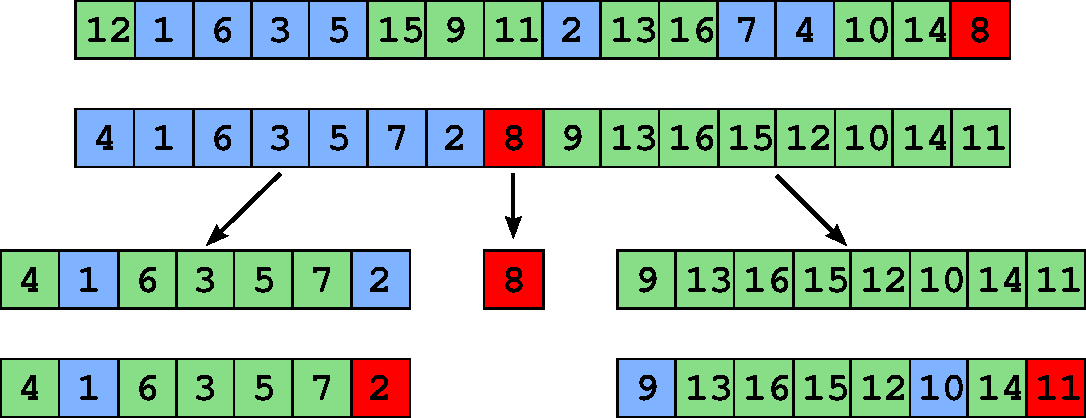
\includegraphics[width=\linewidth]{images/quicksort.pdf}
\end{center}
\end{frame}

\begin{frame}{QuickSort: complexité}
 Le parcours du tableau implique $N-1$ comparaison. Puis on réitère l'opération sur chaque moitié de tableau.
 
 En notant $i$ la position du pivot, la complexité s'écrit:
 $$ {\color{blue} C_{moy}(N)} = {\color{red} N - 1} + {\color{green!50!black} \mathbb{E}[C_{moy}(i-1) + C_{moy}(N-i)]}~~,$$
 
 car le tri du tableau de longueur $N$ implique:
 \begin{itemize}
  \item {\color{red} N - 1 comparaisons pour placer le pivot},
  \item {\color{green!50!black} le tri d'un tableau de longueur $i - 1$ (à gauche du pivot)},
  \item {\color{green!50!black} le tri d'un tableau de longueur $N - i$ (à droite du pivot)}.
 \end{itemize}
\end{frame}

\begin{frame}{QuickSort: complexité}
 Le pivot peut se retrouver à {\color{purple}n'importe quelle position} de {\color{brown}façon équiprobable}:
$$\color{green!50!black} \mathbb{E}[C_{moy}(i-1) + C_{moy}(N-i)] = {\color{brown} \frac{1}{N} \sum_{{\color{purple} p=1}}^{{\color{purple} N}}}  \left[ C_{moy}({\color{purple} p-1}) + C_{moy}({\color{purple} N-p})\right]$$

\uncover<2>{
puis, en réinjectant dans la complexité moyenne:
$$ {\color{blue} C_{moy}(N)} = {\color{red} N - 1 } + {\color{green!50!black} {\color{brown} \frac{1}{N} \sum_{{\color{purple} p=1}}^{{\color{purple} N}}} \left[ C_{moy}({\color{purple} p-1}) + C_{moy}({\color{purple} N-p}) \right]}~~.$$
 }
\end{frame}

\begin{frame}{QuickSort: complexité}

 $$ {\color{blue} C_{moy}(N)} = {\color{red} N - 1 } + {\color{green!50!black} {\color{brown} \frac{1}{N} \sum_{{\color{purple} p=1}}^{{\color{purple} N}}}  C_{moy}({\color{purple} p-1}) + {\color{brown} \frac{1}{N} \sum_{{\color{purple} p=1}}^{{\color{purple} N}}} C_{moy}({\color{purple} N-p})}~~.$$

 \uncover<2->{
 Un changement de variable $q = N - p$ dans la seconde somme donne:
 $$ {\color{blue} C_{moy}(N)} = {\color{red} N - 1} + {\color{green!50!black} \frac{1}{N} \sum_{p=1}^N  C_{moy}(p-1) + \frac{1}{N} \sum_{q=1}^N  C_{moy}(q-1)} $$
 }

 \uncover<3->{
 Autrement dit, la complexité se réécrit:
 $$ {\color{blue} C_{moy}(N)} = {\color{red} N - 1} + {\color{green!50!black} \frac{2}{N} \sum_{p=1}^N  C_{moy}(p-1)}$$
 }
\end{frame}

\begin{frame}{QuickSort: complexité}
 En multipliant par $N$ des deux côtés:
 $$ N {\color{blue} C_{moy}(N)} = N{\color{red} (N - 1)} + {\color{green!50!black} 2 \sum_{p=1}^N  C_{moy}(p-1)}~~~{\color{magenta} (a)}$$
 
 \uncover<2->{En outre, pour un tableau de taille $N-1$, la relation ${\color{magenta} (a)}$ se réécrit:
 $$ (N-1) {\color{blue} C_{moy}(N-1)} = (N-1).{\color{red} (N - 2)} + {\color{green!50!black} 2 \sum_{p=1}^{N-1}  C_{moy}(p-1)}~~.~~{\color{magenta} (b)}$$}
 
 \uncover<3->{
	En calculant $\color{magenta} (a) - (b)$, il vient:
	$$ N {\color{blue} C_{moy}(N)} - (N - 1) {\color{yellow!50!black} C_{moy}(N-1)} = {\color{red} 2N} + {\color{yellow!50!black} 2C_{moy}(N-1)}~~.$$
 }
\end{frame}

\begin{frame}{QuickSort: complexité}
	En simplifiant:
	$$ N{\color{blue} C_{moy}(N)} = {\color{red} 2N} + {\color{yellow!50!black} (N+1) C_{moy}(N-1)}~~.$$
	
	\uncover<2->{On divise par $N(N+1)$:
	$$ \frac{\color{blue} C_{moy}(N)}{N+1} = {\color{red} \frac{2}{N+1}} + {\color{yellow!50!black} \frac{C_{moy}(N-1)}{N}}$$}
	
	\uncover<3->{Puis par récurrence:
	$$ \frac{\color{blue} C_{moy}(N)}{N+1} = {\color{red} \sum_{k=3}^{N+1} \frac{2}{k}} + {\color{yellow!50!black} \frac{C_{moy}(1)}{2}}$$}
\end{frame}

\begin{frame}{QuickSort: complexité}

 Comme:
	$$\color{red} \sum_{k=1}^{N} \frac{1}{k}\underset{N \rightarrow \infty}{\sim} \log(N) $$

\uncover<2>{
 en remplaçant dans la complexité moyenne, on obtient l'équivalence

$${\color{blue} C_{moy}(N)} \underset{N \rightarrow \infty}{\sim} (N+1) {\color{red} log(N)} + (N+1) {\color{yellow!50!black} \frac{C_{moy}(1)}{2}}$$
}
 Finalement:
$$\boxed{C_{moy}(N) = O(N \log(N))}$$

\end{frame}


\subsection{Tri fusion}

\begin{frame}{Tri fusion}

Le principe du tri fusion est proche du tri rapide. L'idée est de couper un tableau en deux, de trier chaque moitié du tableau, puis de remplir un nouveau tableau avec les sous-tableaux triés.

\end{frame}

\begin{frame}
 \frametitle{Tri fusion}

\begin{figure}
\centering
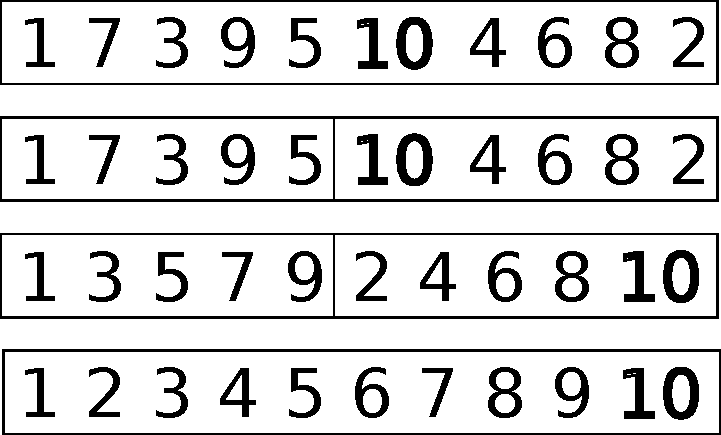
\includegraphics[width = 0.7\linewidth]{./images/fusion.pdf}
\end{figure}
\end{frame}

\begin{frame}
\frametitle{Calcul de la complexité}
\framesubtitle{Tri fusion}

Le parcours du tableau implique $\color{red} N-1$ comparaison. Donc:
$$ {\color{blue} C_N} = {\color{red} (N-1)} + {\color{green!50!black} C_i + C_{N-i-1}}$$
\uncover<2->{En moyenne, $i \simeq \frac{N}{2}$:
$$ {\color{blue} C_N} = {\color{red} N} + {\color{green!50!black} 2 \cdot C_{\frac{N}{2}}}$$}
\uncover<3->{Au rang suivant:
$$ {\color{blue} C_N} = {\color{red} 2N} + {\color{green!50!black} 4 \cdot C_{\frac{N}{4}}}$$}
\uncover<4->{Puis:
$$ {\color{blue} C_N} = {\color{red} k N} + {\color{green!50!black} 2^k \cdot C_{\frac{N}{2^k}}}$$}
\uncover<5->{La récurrence se termine après $k = log_2(N)$ étapes, donc:
$$\boxed{C_N = N \log N + N C_1 = O(N \log N)}$$}
\end{frame}

\begin{frame}
 \frametitle{Tri fusion}
 Le tri fusion est un $O(N\log(N))$ dans tous les cas. Cependant il est en moyenne plus lent que Quicksort, c'est pourquoi ce dernier est le plus utilisé.
\end{frame}

\section{Transformée de Fourier rapide}

\begin{frame}{Transformée de Fourier discrète}
La transformée de Fourier discrète (\emph{Discrete Fourier Transform} ou DFT) est un algorithme central en traitement du signal et des images.

\centering
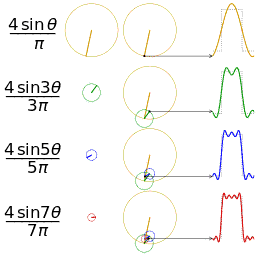
\includegraphics[width=0.5\textwidth]{images/fourier}

\end{frame}

\begin{frame}{DFT: construction (1/2)}
Soit l'espace complexe $\mathbb{C}^N$ et la forme hermitienne:
\[\langle f,g \rangle = \sum_{j=0}^{N-1}f[k]\overline{g[k]}.\]

La famille des vecteur $e_k$:
\[ e_k = \frac{1}{\sqrt{N}}\begin{pmatrix}
e^{\frac{2i\pi}{N} 0\cdot k}, & e^{\frac{2i\pi}{N} 1\cdot k}, & \dots, & e^{\frac{2i\pi}{N} (N-1)\cdot k}
\end{pmatrix}\]
pour $k=0, \ldots, N-1$ est une famille libre orthonormale (donc une base).
\end{frame}

\begin{frame}{DFT: construction (2/2)}
Soit $f$ un tableau de $N$ nombres complexes.
Comme $(e_0,e_1,\dots, e_{N-1})$ est une base, $f$ se décompose de la façon suivante:

\[f = \sum_{j=0}^{N-1} \langle f,e_j \rangle \, e_j\]

Les coefficients de la transformée de Fourier discrète de $f$ sont les coordonnées de $f$ dans cette nouvelle base.
\end{frame}


\begin{frame}{Calcul de la DFT}
	\begin{alertblock}{Expression}
	La transformée de Fourier discrète transforme un tableau $f$ de $N$ nombres complexes en un tableau $DFT(f)$ de même taille par l'opération suivante:
	\[DFT(f)[k] = \langle f,e_j \rangle =  \frac{1}{\sqrt{N}}\sum_{j=0}^{N-1}f[j]e^{-\frac{2i\pi}{N} jk}.\]
	\end{alertblock}
	
	\begin{exampleblock}{Interprétation physique}
	Le coefficient $DFT(f)[k]$ représente l'énergie du signal $f$ à la fréquence $k$. 
	\end{exampleblock}
\end{frame}

\begin{frame}{DFT: transformée inverse}
Soit $f$ un tableau de $N$ nombres complexes.
Comme $(e_0,e_1,\dots, e_{N-1})$ est une base:

\[f = \sum_{j=0}^{N-1} \langle f,e_j \rangle \, e_j\]

ou encore:

\[f = \sum_{j=0}^{N-1} DFT(f)[j] \, e_j\]

\end{frame}
\begin{frame}{DFT: transformée inverse}
\[f = \sum_{j=0}^{N-1} DFT(f)[j] \, e_j\]
\[f[k] = \left( \sum_{j=0}^{N-1} DFT(f)[j] \, e_j \right) [k] \]
\[f[k] = 
\frac{1}{\sqrt{N}}  \sum_{j=0}^{N-1} DFT(f)[j] e^{+\frac{2i\pi}{N} jk}  \]

Notant $IDFT$ la transformée inverse ($IDFT\circ DFT = Id$):

\[f[k] =  IDFT(DFT(f))[k] = \frac{1}{\sqrt{N}}  \sum_{j=0}^{N-1} DFT(f)[j] e^{+\frac{2i\pi}{N} jk} \]
\end{frame}

\begin{frame}{DFT}
Pour résumer, $f$ un tableau de $N$ nombres complexes:
\begin{alertblock}{Discrete Fourier Transform}
\[DFT(f)[k] =  \frac{1}{\sqrt{N}}\sum_{j=0}^{N-1}f[j]e^{-\frac{2i\pi}{N} jk}.\]
\end{alertblock}
\begin{alertblock}{Inverse Discrete Fourier Transform}
\[IDFT(g)[k] =  \frac{1}{\sqrt{N}}\sum_{j=0}^{N-1}g[j]e^{+\frac{2i\pi}{N} jk}.\]
\end{alertblock}
\end{frame}

\begin{frame}{Pourquoi ?}

\begin{block}{Motivation}
La transformée de Fourier transformes les convolutions (= opérations de filtrage) en multiplication. Il est bien plus rapide de faire une multiplication dans l'espace de Fourier qu'une convolution dans l'espace initial.
\end{block}

\only<1>{\centering 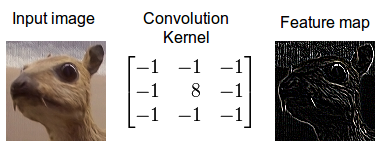
\includegraphics[width=0.8\textwidth]{images/convolution}}

\only<2>{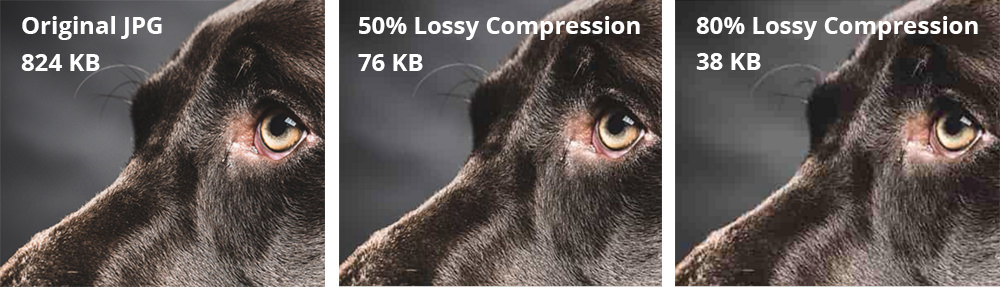
\includegraphics[width=\textwidth]{images/jpeg_compression}}

\end{frame}

\begin{frame}{DFT: complexité a priori}
\[DFT(f)[k] =  \frac{1}{\sqrt{N}}\sum_{j=0}^{N-1}f[j]e^{-\frac{2i\pi}{N} jk}.\]
Calculer un terme: $O(N)$.

\vspace{0.5cm}
Calculer tous les termes: $ O(N^2)$
\end{frame}

\begin{frame}{Fast Fourier Transform}

\begin{center}
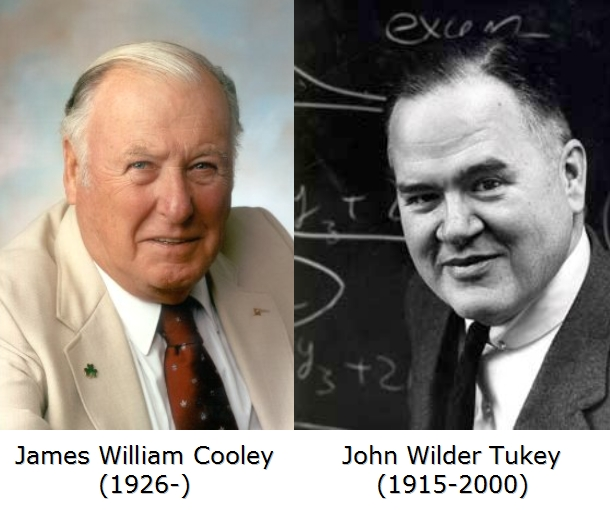
\includegraphics[width=0.5\textwidth]{images/cooley_tukey.jpg}
\end{center}

La FFT est un algorithme introduit par Cooley and Tukey en 1965. Elle permet de calculer la DFT en temps $N \log(N)$.

Elle utilise une approche \textbf{diviser pour régner}.

\end{frame}

\begin{frame}{FFT: algorithme}
On sépare la somme dans la DFT en indices {\color{red} pairs} et {\color{blue} impairs}:
\[\sqrt{N}~DFT(f)[k] =
{\color{red}\sum_{j=0}^{N/2-1}f[2j]e^{-\frac{2i\pi}{N} (2j)k}} +
{\color{blue} \sum_{j=0}^{N/2-1}f[2j+1]e^{-\frac{2i\pi}{N} (2j+1)k}},\]
dont on déduit facilement
\[\sqrt{N}~DFT(f)[k] =
{\color{red}\sum_{j=0}^{N/2-1}f[2j]e^{-\frac{2i\pi}{N/2} jk}} +
{\color{green!50!black} e^{-\frac{2i\pi}{N}k}}
{\color{blue} \sum_{j=0}^{N/2-1}f[2j+1]e^{-\frac{2i\pi}{N/2} jk}}.\]
\end{frame}

\begin{frame}{FFT: algorithme}
On retrouve en fait le calcul de la transformée de Fourier discrète sur les deux sous-tableaux:
\begin{equation}
\sqrt{N} DFT(f)[k] = \sqrt{\frac{N}{2}}
\left(
{\color{red} DFT(f_\text{pair})[k]} + {\color{green!50!black} e^{-\frac{2i\pi}{N}k}} {\color{blue} DFT(f_\text{impair})[k]}
\right)
\end{equation}
\begin{itemize}
	\item $f_\text{pair}$ est le sous-tableau des indices pairs de $f$: \mintinline{python}{f[0:n:2]};
	\item $f_\text{impair}$ est celui des indices impairs: \mintinline{python}{f[1:n:2]}.
\end{itemize}
\end{frame}

\begin{frame}{FFT: algorithme}
\begin{equation}
\sqrt{N} DFT(f)[k] = \sqrt{\frac{N}{2}}
\left(
{\color{red} DFT(f_\text{pair})[k]} + {\color{green!50!black} e^{-\frac{2i\pi}{N}k}} {\color{blue} DFT(f_\text{impair})[k]}
\right)
\end{equation}
Le problème est alors de:
\begin{enumerate}
    \item Calculer la DFT des indices pairs de $f$.
    \item Calculer la DFT des indices impairs de $f$.
    \item Combiner en $O(N)$ les deux suivant la formule ci-dessus.
\end{enumerate}
\end{frame}

\begin{frame}{Complexité}
Le calcul de complexité de la FFT (\emph{Fast Fourier Transform}) est analogue à celle du tri fusion:
\begin{itemize}
    \item calcul sur les tableau de taille $N/2$
    \item relation de récurrence $C(N) \approx N + 2*C(\frac{N}{2})$
    \item complexité en $O(N \log(N))$
\end{itemize}
\end{frame}

\begin{frame}{Implémentation}
$$
\sqrt{N}~DFT(f)[k] = \sqrt{\frac{N}{2}}
\left(
{\color{red} DFT(f_{0:2:N-2})[k]} + {\color{green!50!black} e^{-\frac{2i\pi}{N}k}} {\color{blue} DFT(f_{1:2:N-1})[k]}
\right)
$$
\only<1>{
Relation de récurrence:
\begin{enumerate}
\item Calculer la DFT des indices pairs de $f$.
\item Calculer la DFT des indices impairs de $f$.
\item Combiner en $O(N)$ les deux suivant la formule ci-dessus.
\end{enumerate}
}
\only<2>{
Les sous DFT sont de longueur $N/2$, donc définies pour $0 \leq k \leq N/2$.
En remarquant que:
$$\exp\left(-\frac{2i\pi}{N/2}j(k+N/2)\right) =  \exp\left(-\frac{2i\pi}{N/2}jk\right)$$
$$\exp\left(-\frac{2i\pi}{N}(k+N/2)\right) =  \exp\left(-\frac{2i\pi}{N}k\right)$$
on s'aperçoit qu'il y a périodicité de la DFT:
$$DFT_\text{paire}\left[k + \frac{N}{2}\right] = DFT_\text{paire}[k],$$
$$DFT_\text{impaire}\left[k + \frac{N}{2}\right] = DFT_\text{impaire}[k]~~.$$
}
\only<3>{
\begin{enumerate}
\item Calculer la DFT des indices pairs de $f$.
\item Calculer la DFT des indices impairs de $f$.
\item Combiner en $O(N)$ les deux suivant la formule ci-dessus.
\begin{itemize}
\item Copier $f$ dans un tableau temporaire \texttt{buffer}. On a dans les indices pairs et impairs les résultats des sous-DFT (non normalisées).
\item Boucle de $k=0$ à $N/2-1$:\\
\begin{align*}
f[k] \leftarrow \texttt{buffer}[2*k]&+e^{-\frac{2i\pi}{N}k}\,\texttt{buffer}[2*k+1]\\
f[k+N/2] \leftarrow \texttt{buffer}[2*k]&-e^{-\frac{2i\pi}{N}k}\,\texttt{buffer}[2*k+1].
\end{align*}
\end{itemize}
\end{enumerate}

}
\end{frame}

\begin{frame}{En pratique}
\begin{itemize}
\item Le facteur $\color{green!50!black} t_k=e^{-\frac{2i\pi}{N}k}$ est appelé \emph{twiddle}. On en fait un calcul rapide par la relation de récurrence de suite géométrique $t_{k+1} = r\,t_k$, dont la raison $r=e^{-\frac{2i\pi}{N}}$ est pré-calculée.
\item On alloue une seule fois \texttt{buffer} et on le passe dans les arguments de la fonction récursive.
\end{itemize}
\end{frame}

\begin{frame}{Dérivation}
Il est possible de définir un équivalent de dérivation pour la DFT.

Soit $e_j(x) = \frac{1}{\sqrt{N}}\exp(\frac{2i\pi}{N}jx)$.
Pour $k \in \mathbb{N}$:  $e_j(k)=e_j[k]$ 

Soit $f$ la fonction périodique:
\[f(x) = \sum_j DFT(f)[j]e_j(x),\]

et $f(k) = f[k]$: 

\[f'(x) = \sum_j DFT(f)[j]e_j'(x)=\sum_j \frac{2i\pi j}{N}DFT(f)[j]e_j(x).\]

Puis: 
\[DFT(f')[j] = \frac{2i\pi j}{N}DFT(f)[j].\]
\end{frame}

\begin{frame}{Dérivation}

Pour les fonctions réelles: il faut que $f'$ soit réelle.

\[
DFT(f')[j] =
\begin{cases}
\frac{2i\pi}{N}j\,DFT(f)[j] & \text{pour }0\leq j<N/2\\
0 & \text{pour }j=N/2\\
\frac{2i\pi}{N}(j-N)\,DFT(f)[j] & \text{pour }N/2<j<N
\end{cases}
\]

Cette relation est utile pour résoudre certaines équations aux dérivées partielles. En particulier, l'équation de Poisson que nous allons résoudre en TP.

\end{frame}

\section{Codons!}
\begin{frame}{Codons!}
	TP long: transformée de Fourier rapide et éditeur de Poisson.
	
	\begin{block}{Idée}
	Comment copier/coller un morceau d'image dans une autre? Pour que les transitions soient naturelles, il faut que les variations d'intensité au niveau de la frontière soient égales: c'est l'équation de Poisson.
	
	Cette équation est simple à résoudre dans l'espace de Fourier. Il suffit ensuite de récupèrer l'image lissée en appliquant la transformée de Fourier inverse.
	\end{block}
\end{frame}
\end{document}
